\appendix
\section{Code Snippets}
\label{app:code_snippets}
\begin{figure}[H]
	\centering
	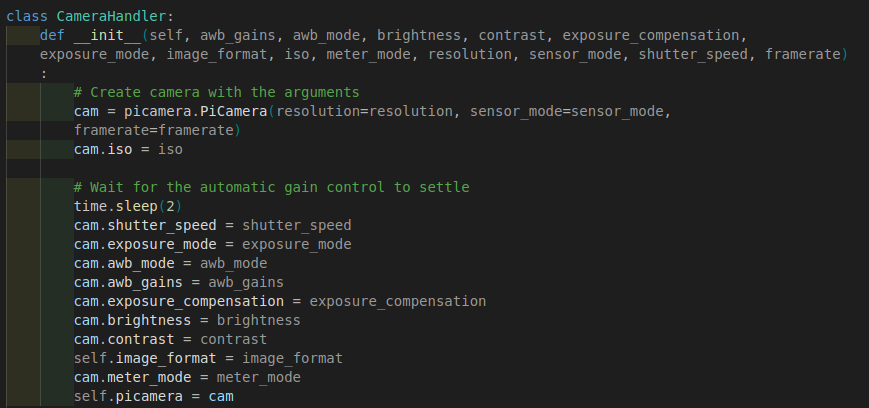
\includegraphics[width=\textwidth]{Images/Code Screenshots/camerahandler.png}
	\caption{CameraHandler class initialization.}
	\label{fig:code_camerahandler}
\end{figure}

\section{Technical Challenges}
\paragraph{Pi out of memory on image capture}
Context: tweaking camera settings, leading to larger size images
Error: mal port enable failed to enable connected port... Out of resources.
Solution: allocating more memory to the GPU by going through raspi-config Performance Options -> GPU Memory

\paragraph{AWB Gains}
Context: setting picamera.awg gains has no effect
Error: no change
Solution: set awb gains after awb mode has been set to off, and capture an image. The control seems to not set before after capturing an image. Thus, setting these values and then checking the values, it might seem the modification has not been made altough it will show on the images.

\section{Camera Settings Explanation}
\label{app:camera_settings_explanation}
\begin{itemize}
	\item $awb\_gains$ - Set the auto white balance gains red and blue. Set as a (red, blue) set. Each value may range from 0.0 to 8.0. Typical is 0.9-1.9. Only has an effect when $awb\_mode$ is 'off'. IMPORTANT: awb and exposure mode must be set to off BEFORE setting the $awb\_gains$.
	\item $awb\_mode$ - Auto white balance. Default is auto. Disabling auto white balance mode allows for manual setting of AWB gains, ensuring consistent image color temperature. 'off' 'auto' 'sunlight' 'cloudy' 'shade' 'tungsten' 'fluorescent' 'incandescent' 'flash' 'horizon'
	\item \textit{brightness} - Adjusts the post-processing brightness of the image. Default is 50, representing no adjustment. 0 to 100.
	\item contrast - Adjusts the post-processing contrast of the image. Default is 0, representing no adjustment. -100 to 100.
	\item $exposure\_compensation$- Adjusts the exposure compensation level. Range is -25 to 25. Default is 0.
	\item $exposure\_mode$ - Disabling auto-exposure allows for manual control over exposure settings. 'off' 'auto' 'night' 'nightpreview' 'backlight' 'spotlight' 'sports' 'snow' 'beach' 'verylong' 'fixedfps' 'antishake' 'fireworks'.
	\item $exposure\_speed$ - Indicates the effective exposure speed, which may differ from the set shutter speed after adjustments.
	\item \textit{framerate} - Sets the number of frames per second captured by the camera.
	\item \textit{iso} - Sets the ISO sensitivity of the camera sensor. Values: 100, 200, 320, 400, 500, 640, 800. 0 is auto.
	\item $metering\_mode$ - Sets the metering mode. 'average' 'spot' 'backlit' 'matrix'. Backlit is the largest area. Default is average.
	\item $sensor\_mode$ - Controls the sensor mode, where '3' typically corresponds to standard image capturing.
	\item $shutter\_speed$ - Sets the shutter speed in microseconds. 0 to 6000000. Default 0. 0 is auto. Max 6s.
	\item \textit{resolution} - Sets the resolution of the image frame.
\end{itemize}

\section{TinyML and Frugal Devices}
\label{app:tinyML}
As mentioned in Section \ref{sec:scope_tinyML}, TinyML is when machine learning models are aimed at deployment to heavily resource constrained environments, e.g. what is called frugal devices. These are devices where the microcontroller units (MCUs) are accompanied by memory measured in kilobytes, and processor speeds measured in megahertz. 

Machine learning networks applied to tiny robots are subject to challenges from size, weight, area, and power (SWAP) (\cite{ne2022robotstinymlconstraints}). Many of the same challenges apply even in applications where the SWAP challenges are not the main concerns. \citeauthor{ra2023reformabletinyml} mentions the open challenges and future directions of the next generation tinyML. Catastrophic forgetting, which is when information from previous tasks while learning new ones are forgotten, are a result of the frugal devices' computational resources and memory. The first recommendation for future directions from the authors is to investigate fog computing as a means to offload tasks from the frugal devices.

\citeauthor{ma2023tinyML_speech_recognition} (\citeyear{ma2023tinyML_speech_recognition}) explore the ways of speech processing on microcontrollers to improve car AI systems. They employed their trained and optimized model to an Arduino Nano 33 BLE. The model achieved accuracies in above 85 percent on recognizing whether the voice was that of an adult or a child, and to detect whether the speech was a replay (synthetic) or "live". 

Furthermore, \citeauthor{ra2023reformabletinyml} discuss some of the challenges in industrial IoT environments with several smart object devices, where having the devices share a collective dataset of anomalies within a manufacturing environment would be advantageous for utilizing collective learning to improve the ML models in each of the devices (\citeyear{ra2023reformabletinyml}). This means the devices will all learn from observations of the other devices, such that the training period from when a network of devices is deployed within a new environment to when they are fully functioning with regards to accuracy in their predictions is reduced. See more about this in section \ref{sec:federated_learning} about federated learning as a way of implementing a collective learning network for the edge devices.
